\textbf{5.1.1.} 一长直导线载有电流 I，试求它上面长为 $l_{1} + l_{2}$ 的一段电流在离它为 r 处的 P 点（图 5.1.1）所产生的磁感强度 B；当 $l_{1}$ 和 $l_{2}$ 都趋于 $\infty$ 时，结果如何？

\vfill

\textbf{5.1.2.} 一长直导线载有电流 $I$ ，试求它上面长为 $l$ 的一段电流在中垂面上距离为 $r$ 处的 $P$ 点（图5.1.2）所产生的磁感强度 $\pmb{B}$ ；当 $l \to \infty$ 时结果如何？

\vfill

\newpage

\textbf{5.1.3.} 一条很长的直输电线,载有 100A 的电流,试问在离它半米处,它产生的磁感强度有多大?

\vfill

\textbf{5.1.4.} 一条很长的载流直导线,在离它 1cm 处产生的磁感强度为 1Gs,试问它所载的电流有多大?

\vfill

\newpage

\textbf{5.1.5.} 一条很长的直导线载有电流 I; 在这导线上套有一个圆环, 环的轴线与导线重合, 环的横截面积是边长分别为 b 和 c 的长方形, 环的内半径为 a, 环的一半如图 5.1.5 所示. 试求通过这圆环的横截面的磁通量 $\Phi = \int_{S} B \cdot dS$ .
\begin{center}
    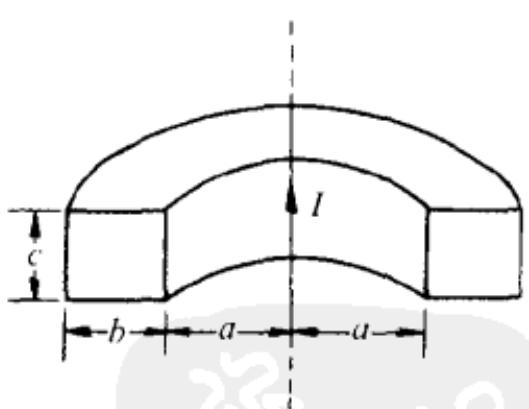
\includegraphics[width=0.5\linewidth]{figures/fig_5_1_5.jpg}
\end{center}

\vfill

\textbf{5.1.6.} 载有电流 I 的无穷长直导线在一处折成直角, 如图 5.1.6 所示. P 为线外一点, 在折线的延长线上, 到折点的距离为 a. 试求 P 点的磁感强度 B, 并计算 I = 20 安培, a = 2.0 厘米时 B 的大小.

\vfill

\newpage

\textbf{5.1.7.} 载有电流 $I$ 的导线构成边长为 $2a$ 的正方形, 如图 5.1.7(1) 所示. (1) 试求正方形轴线上离中心 $O$ 为 $r$ 处的磁感强度 $\pmb{B}$ 和磁场强度 $\pmb{H}$ ; (2) 当 $I = 5.0\mathrm{A}$ , $a = 4.0\mathrm{cm}, r = 10\mathrm{cm}$ 时, 试计算 $\pmb{B}$ 和 $\pmb{H}$ 的值.

\vfill

\textbf{5.1.8.} 载有电流 $I$ 的导线构成边长为 $a$ 和 $b$ 的长方形, 如图 5.1.8(1) 所示. 试求轴线上离中心 $O$ 为 $r$ 处的磁感强度 $\pmb{B}$ 以及 $r \gg a$ 和 $b$ 处 $\pmb{B}$ 的值.

\vfill

\newpage

\textbf{5.1.9.} 载有电流 $I$ 的导线构成一等边三角形, 每边长为 $2a$ , 试求这三角形轴线上离中心为 $r$ 处 $P$ 点[图5.1.9(1)]的磁感强度 $\pmb{B}$ 以及 $r \gg a$ 处 $\pmb{B}$ 的值.
\begin{center}
    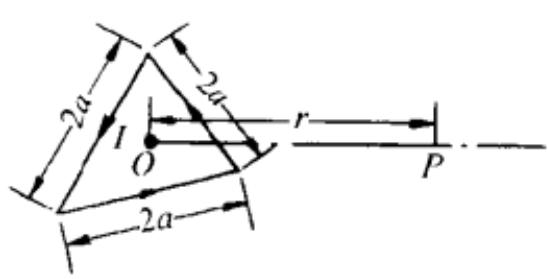
\includegraphics[width=0.5\linewidth]{figures/fig_5_1_9.jpg}
\end{center}

\vfill

\textbf{5.1.10.} 在无线电或电子仪器里,通常都把来回线(即载有大小相等而方向相反的电流的外表绝缘线)并在一起或缠扭成一条,以减少它们在周围产生的磁场,试说明这样做的道理.

【解答】根据Biot-Savart定理，靠得很近而方向相反的两条平行线电流，在它们外面任一点产生的磁感强度近乎大小相等而方向相反，故合成的磁感强度几乎为零.

图5.1.11
\begin{center}
    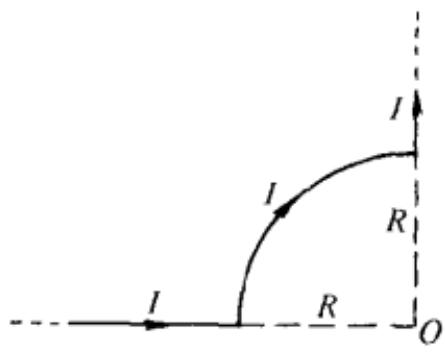
\includegraphics[width=0.5\linewidth]{figures/fig_5_1_10.jpg}
\end{center}

\vfill

\newpage

\textbf{5.1.11.} 一条载有电流 I 的无穷长直导线，在一处弯折成半径为 R 的 $\frac{1}{4}$ 圆弧，如图 5.1.11 所示。试求这 $\frac{1}{4}$ 圆弧中心 O 点的磁感强度 B。

\vfill

\textbf{5.1.12.} 一条载有电流 I 的无穷长直导线, 在一处弯折成半径为 R 的半圆弧, 如图 5.1.12 所示. 试求半圆弧中心 O 点的磁感强度 B.

\vfill

\newpage

\textbf{5.1.13.} 一条载有电流 I 的无穷长直导线, 在一处弯折成

图5.1.12

半径为 R 的半圆弧, 试求这半圆弧轴线上离中心 O 为 r 处的磁感强度 B [图 5.1.13(1)], 并计算 $R = 10 \, cm, r = 40 \, cm, I = 4.0$ 安培时 B 的值.

\vfill

\textbf{5.1.14.} (1) 一条载有电流 $I$ 的无穷长直导线在一处分叉成两路后又合而为一, 这两路是半径为 $R$ 的圆, 如图 5.1.14(1) 所示. 试求圆心的磁感强度 $\pmb{B}$ . (2) 一条载有电流 $I$ 的无穷长直导线在一处弯成半径为 $R$ 的圆形, 如图 5.1.14(2) 所示, 由于导线表面有绝缘层, 所以在接触处并不短路. 试求圆心的磁感强度 $\pmb{B}$ .

(1)

(2)
图5.1.14
\begin{center}
    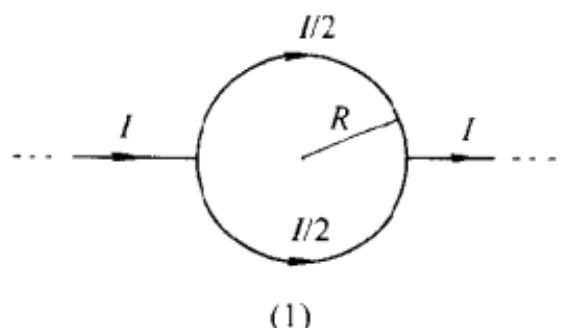
\includegraphics[width=0.5\linewidth]{figures/fig_5_1_14_1.jpg}
\end{center}
\begin{center}
    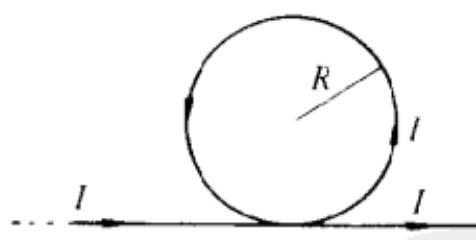
\includegraphics[width=0.5\linewidth]{figures/fig_5_1_14_2.jpg}
\end{center}

\vfill

\newpage

\textbf{5.1.15.} 一段载有电流 I 的导线弯折成如图 5.1.15(1) 所示的环路, 两对边是相距为 2a 的平行直线, 另外两对边是以 O 为中心、R 为半径的两段圆弧. 试求 O 点的磁感强度 B.

\vfill

\textbf{5.1.16.} 一载有电流 I 的导线弯成半径为 R 的圆弧, 弧的两端之间则是一段直线, 对圆心 O 的张角为 $2\theta$ , 如图 5.1.16(1) 所示. 试求圆心的磁感强度 B.

\vfill

\newpage

\textbf{5.1.17.} 一载有电流 $I$ 的导线弯折成如图5.1.17所示的环路，其中一部分是半径为 $r$ 的四分之三圆弧，另一部分是半径为 $R$ 的四分之一的同心圆弧，这两圆弧在同一平面内，它们的两端都以直线联接。当这回路中载有电流 $I$ 时，试求圆心 $O$ 的磁感强度。

图5.1.17
\begin{center}
    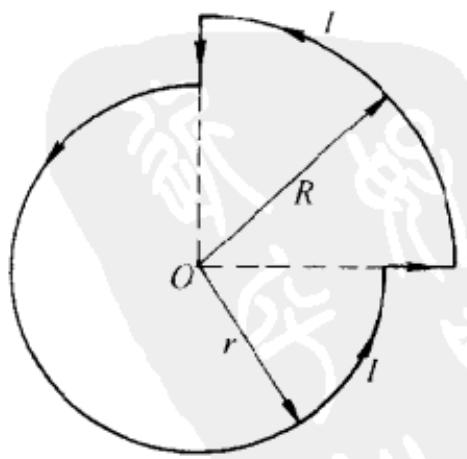
\includegraphics[width=0.5\linewidth]{figures/fig_5_1_17.jpg}
\end{center}

\vfill

\textbf{5.1.18.} 一载有电流 I 的导线弯折成如图 5.1.18(1) 所示的平面环路, 其中 FABCD 是边长为 b 的正方形的一部分, DEF 是半径为 a 的四分之三圆弧, 圆弧的中心 O 在正方形延长线的顶点. 试求 O 点的磁感强度 B.

\vfill

\newpage

\textbf{5.1.19.} 一无穷长导线载有电流 I，在中间弯折成一半径为 R 的半圆弧，其余部分则与圆弧的轴线平行，如图 5.1.19 所示。试求圆弧中心 O 的磁感强度 B，并计算 I = 8.0A、R = 10.0cm 时 B 的值。

\vfill

\textbf{5.1.20.} 一载有电流 I 的导线弯成半径为 R 的圆形, 如图 5.1.20 所示. 试求轴线上离圆心 O 为 r 处的磁感强度 B, 并计算 $R = 11 \, cm, I = 14 \, \Lambda$ 时, r = 0 和 r = 10cm 处 B 的值.

\vfill

\newpage

\textbf{5.1.21.} 一载流圆线圈共有 10 匝, 每匝的电流都是 10A, 线圈的直径为 10cm, 试求线圈中心磁感强度 B 和磁场强度 H 的值.

\vfill

\textbf{5.1.22.} 一载有电流 $I$ 的导线弯成半径为 $\alpha$ 的圆形, 如图5.1.22(1)所示. 试求: (1) $\pmb{r}$ 处 $P$ 点的磁感强度 $\pmb{B}$ 的表达式; (2) $r \gg a$ 处 $\pmb{B}$ 在 $\pmb{r}$ 方向上的分量 $B_{r}$ 和 $\theta$ 方向上的分量 $B_{\theta}$ .

图5.1.22(1)
\begin{center}
    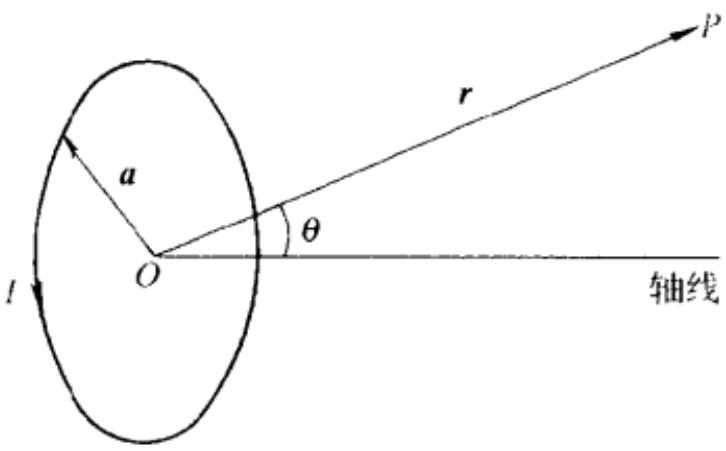
\includegraphics[width=0.5\linewidth]{figures/fig_5_1_22.jpg}
\end{center}

\vfill

\newpage

\textbf{5.1.23.} 两载流圆线圈共轴, 半径分别为 $R_{1}$ 和 $R_{2}$ , 电流分别为 $I_{1}$ 和 $I_{2}$ , 电流方向相同, 两圆心 $O_{1}$ 和 $O_{2}$ 相距为 $2a$ , 联线的中点为 $O$ , 如图 5.1.23 所示. 试分别求轴线上离 O 为 $r_{1}$ 处 $P_{1}$ 点和离 O 为 $r_{2}$ 处 $P_{2}$ 点的磁感强度 $B_{1}$ 和 $B_{2}$ .

\vfill

\textbf{5.1.24.} 两载流圆线圈共轴, 半径分别为 $R_{1}$ 和 $R_{2}$ , 电流分别为 $I_{1}$ 和 $I_{2}$ , 电流方向相反, 两圆心 $O_{1}$ 和 $O_{2}$ 相距为 2a, 联线的中点为 O, 如图 5.1.24 所示. 试求轴线上离 O 为 r 处的磁感强度 B.

\vfill

\newpage

\textbf{5.1.25.} 两个相同的圆线圈, 半径都是 R, 载有相同的电流 I, 共轴放置, 两圆心 $O_{1}$ 和 $O_{2}$ 相距为 a, 如图 5.1.25 所示, O 是 $O_{1}$ 和 $O_{2}$ 联线的中点. 以 O 为原点, 轴线为 x 轴. (1) 试求轴线上坐标为 x 处的磁感强度 B; (2) 试证明: 当 a = R 时, O 处的磁场近乎均匀磁场.

图5.1.25

$R_{1} - R_{2} - R, I_{1} = I_{2} = I$ ，代入5.1.23题的式(6)，并将其中的 $a$ 换成 $\frac{a}{2}$ ，便得本题所要求的磁感强度

$$
\boldsymbol {B} = \frac {\mu_ {0} I R ^ {2}}{2} \left\{\frac {1}{\left. \left(x + \frac {a}{2}\right) ^ {2} + R ^ {2} \right] ^ {3 / 2}} + \frac {1}{\left[ \left(x - \frac {a}{2}\right) ^ {2} + R ^ {2} \right] ^ {3 / 2}} \right\rangle \boldsymbol {e} _ {1}\tag{1}
$$

式中 $e_{1}$ 是 $O_{1}O_{2}$ 方向上的单位矢量.

(2) 在 x=0 处 (即 O 点), 磁感强度 $B(0)$ 的大小为

$$
B (0) = \frac {8 \mu_ {0} I R ^ {2}}{(a ^ {2} + 4 R ^ {2}) ^ {3 / 2}}\tag{2}
$$

由式(1)和 $x$ 处 $\pmb{B}$ 的大小 $B(x)$ 是连续的，故在 $x = 0$ 附近， $B(x)$ 可由Taylor展开为

$$
B (x) = B (0) + \left(\frac {\mathrm{d} B}{\mathrm{d} x}\right) _ {0} x + \frac {1}{2 !} \left(\frac {\mathrm{d} ^ {2} B}{\mathrm{d} x ^ {2}}\right) _ {0} x ^ {2} + \frac {1}{3 !} \left(\frac {\mathrm{d} ^ {3} B}{\mathrm{d} x ^ {3}}\right) _ {0} x ^ {3} + \dots\tag{3}
$$

由式(1)得

$$
\frac {\mathrm{d} B (x)}{\mathrm{d} x} = - \frac {3 \mu_ {0} I R ^ {2}}{4} \left\{\frac {2 \left(x + \frac {a}{2}\right)}{\left[ \left(x + \frac {a}{2}\right) ^ {2} + R ^ {2} \right] ^ {5 / 2}} + \frac {2 \left(x - \frac {a}{2}\right)}{\left[ \left(x - \frac {a}{2}\right) ^ {2} + R ^ {2} \right] ^ {5 / 2}} \right\}
$$

$$
= - \frac {3 \mu_ {0} I R ^ {2}}{2} \left\{\frac {x + \frac {a}{2}}{\left[ (x + \frac {a}{2}) ^ {2} + R ^ {2} \right] ^ {5 / 2}} + \frac {x - \frac {a}{2}}{\left[ (x - \frac {a}{2}) ^ {2} + R ^ {2} \right] ^ {5 / 2}} \right\}\tag{4}
$$

$$
\begin{array}{l} \frac {\mathrm{d} ^ {2} B (x)}{\mathrm{d} x ^ {2}} = - \frac {3 \mu_ {0} I R ^ {2}}{2} \left\{\frac {1}{\left[ \left(x + \frac {a}{2}\right) ^ {2} + R ^ {2} \right] ^ {5 / 2}} + \frac {1}{\left[ \left(x - \frac {a}{2}\right) ^ {2} + R ^ {2} \right] ^ {5 / 2}} \right. \\ \left. - \frac {5 \left(x - \frac {a}{2}\right) ^ {2}}{\left[ \left(x + \frac {a}{2}\right) ^ {2} + R ^ {2} \right] ^ {7 / 2}} - \frac {5 \left(x - \frac {a}{2}\right) ^ {2}}{\left[ \left(x - \frac {a}{2}\right) ^ {2} + R ^ {2} \right] ^ {7 / 2}} \right\} \end{array}\tag{5}
$$

当 $x = 0$ 时，由式(4)、(5)得

$$
\left(\frac {\mathrm{d} B}{\mathrm{d} x}\right) _ {0} = 0\tag{6}
$$

$$
\left(\frac {\mathrm{d} ^ {2} B}{\mathrm{d} x ^ {2}}\right) _ {0} = - \frac {3 \mu_ {0} I R ^ {2} (R ^ {2} - a ^ {2})}{\left[ \left(\frac {a}{2}\right) ^ {2} + R ^ {2} \right] ^ {7 / 2}}\tag{7}
$$

当 $x = 0$ 且 $R = a$ 时，由式(7)得

$$
\left(\frac {\mathrm{d} ^ {2} B}{\mathrm{d} x ^ {2}}\right) _ {0} = 0\tag{8}
$$

将式(6)、(8)代入式(3)得:在 R=a 和 x=0 时有

$$
B (x) = B (0) + \frac {1}{3 !} \left(\frac {\mathrm{d} ^ {3} B}{\mathrm{d} x ^ {3}}\right) _ {0} x ^ {3} + \dots\tag{9}
$$

在 x 很小的范围内, $x^{3}$ 及高次项都可以略去, 故得

$$
B (x) \approx B (0)\tag{10}
$$

即在 $x = 0$ 附近，磁感强度 $\pmb{B}(x)$ 近乎常矢量 $\pmb{B}(0)$ ，所以 $O$ 处的磁场近乎均匀磁场。

\vfill

\textbf{5.1.26.} 表面绝缘的细导线密绕成一个平面环带, 共有 N 匝, 内外半径分别为 a 和 b, 如图 5.1.26 所示. 当导线中载有电流 I 时, 将每匝中的电流都当作圆电流, 试求环带中心 O 的磁感强度.

\vfill

\newpage

\textbf{5.1.27.} 表面绝缘的细导线绕成一个半径为 $R$ 的平面圆盘，一头在盘中心，一头在盘边缘，沿半径每单位长度为 $n$ 匝，如图5.1.27所示.当导线中载有电流 $I$ 时，将每匝电流都当作圆电流，试求圆盘轴线上离盘心为 $r$ 处 $P$ 点的磁感强度 $\pmb{B}$

图5.1.27

\vfill

\textbf{5.1.28.} 如图 5.1.28, 一半径为 R 的平面圆盘电流, 电流的方向与圆的半径垂直, 沿半径单位长度的电流为 I. 试证明: 它的轴线上离中心为 r 处 P 点的磁感强度为 $B=\frac{\mu_{0}I}{2}\left[\arcsin h(\tan\alpha)-\sin\alpha\right]e_{I}$ ，式中 $\alpha$ 是圆的半径对 P 点所张的角度， $e_{I}$ 是 I 的右旋进方向上（即沿轴线向右）的单位矢量.

\vfill

\newpage

\textbf{5.1.29.} 由表面绝缘的细导线密绕而成的螺线管半径为 R，长为 l，单位长度的匝数为 n，导线中的电流为 I。(1)试求轴线上离管中心为 r 处[图 5.1.29(1)]的磁感强度 B；(2)分别求 r=0 和 $l=\infty$ 时 B 的值.

图5.1.29(1)
\begin{center}
    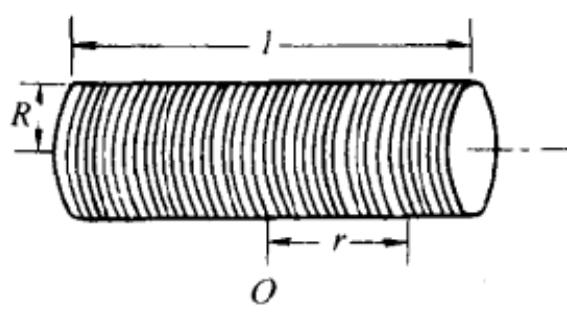
\includegraphics[width=0.5\linewidth]{figures/fig_5_1_29.jpg}
\end{center}

\vfill

\textbf{5.1.30.} 一很长的螺线管由外皮绝缘的细导线密绕而成,每厘米有35匝,导线中的电流为2.0A.试求这螺线管轴线上管中心和管端的磁感强度B的值.

\vfill

\newpage

\textbf{5.1.31.} 一螺线管长 $1.0\mathrm{m}$ , 平均直径为 $3.0\mathrm{cm}$ , 它有五层绕组, 每层有 850 匝, 导线中的电流为 5.0A. (1) 试求管中心的磁感强度 $\pmb{B}$ 的大小; (2) 设管中心横截面上 $\pmb{B}$ 是均匀的, 试求通过该截面的磁通量 $\Phi$ .

\vfill

\textbf{5.1.32.} 一长为 l 的螺线管, 半径为 R, 由表面绝缘的细导线密绕而成, 共有 N 匝. 当通过导线的电流为 I 时, 试求轴线上 P 点的磁场强度 H, P 到一端的距离为 r, 如图 5.1.32(1) 所示.

\vfill

\newpage

\textbf{5.1.33.} 球形线圈是由表面绝缘的细导线在半径为 $R$ 的球面上沿一固定直径密绕而成，沿该直径单位长度的匝数为 $n$ ，并且各处的 $n$ 都相同。当导线中载有电流 $I$ 时，试求：(1)球心 $O$ 的磁感强度 $\pmb{B}_0$ ；(2)该直径端点 $A$ 的磁感强度 $\pmb{B}_A$ 。

\vfill

\textbf{5.1.34.} 球形球圈是由表面绝缘的细导线在半径为 R 的球面上沿一固定直径密绕而成, 沿该直径单位长度的匝数为 n, 并且各处的 n 都相同. 当导线中载有电流 I 时, 试求该直径上离球心为 r 处的磁感强度 B.

\vfill

\newpage

\textbf{5.1.35.} 一载有电流 I 的无穷长导线弯成抛物线, 如图 5.1.35 所示, 焦点到顶点的距离为 a. 试求焦点的磁感强度 $B_{F}$ .

\vfill

\textbf{5.1.36.} 一载有电流 I 的导线弯成椭圆形, 椭圆的方程为 $\frac{x^{2}}{a^{2}} + \frac{y^{2}}{b^{2}} = 1$ , 如图 5.1.36 所示. 试求 I 在焦点 F 产生的磁感强度 $B_{F}$ .

\vfill

\newpage

\textbf{5.1.37.} 一载有电流 I 的导线弯成椭圆形, 椭圆的方程为 $\frac{x^{2}}{a^{2}} + \frac{y^{2}}{b^{2}} = 1, a > b$ , 如图 5.1.37(1) 所示. 试求 I 在椭圆中心 O 产生的磁感强度 $B_{0}$ .

\vfill

\textbf{5.1.38.} 电流 I 沿双曲线流动, 双曲线方程为

$$
\frac {x ^ {2}}{a ^ {2}} - \frac {y ^ {2}}{b ^ {2}} = 1
$$

如图 5.1.38(1) 所示. 试求 I 在焦点 F 产生的磁感强度 $B_{F}$ .

\vfill

\newpage

\textbf{5.1.39.} 宽为 $a$ 的无穷长直导体薄片载有电流 $I, I$ 沿片长的方向流动，并均匀分布在横截面上。通过片的中线并与片的表面垂直的平面上有一点 $P, P$ 到片的距离为 $r$ ，如图5.1.39(1)所示。设片的厚度可略去不计，试求 $P$ 点的磁感强度 $\pmb{B}$ 。

\vfill

\textbf{5.1.40.} 一无穷长直导体薄片宽为 $a = a_{1} + a_{2}$ ，载

图 5.1.39(2)

有电流 I, I 沿片长方向流动, 并均匀分布在横截面上. 片外一点 P 到片的距离为 r, P 在片上的垂足为 S, 如图 5.1.40(1) 所示. 设片的厚度可略去不计, 试求 P 点的磁感强度 B.

图5.1.40(1)

图5.1.40(2)
\begin{center}
    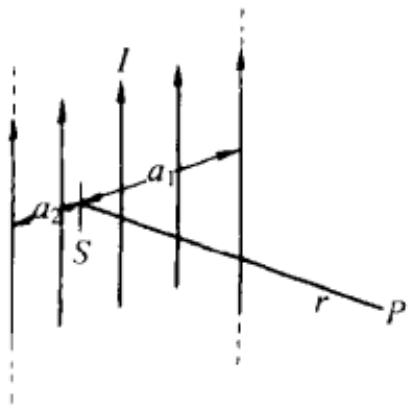
\includegraphics[width=0.5\linewidth]{figures/fig_5_1_40_1.jpg}
\end{center}
\begin{center}
    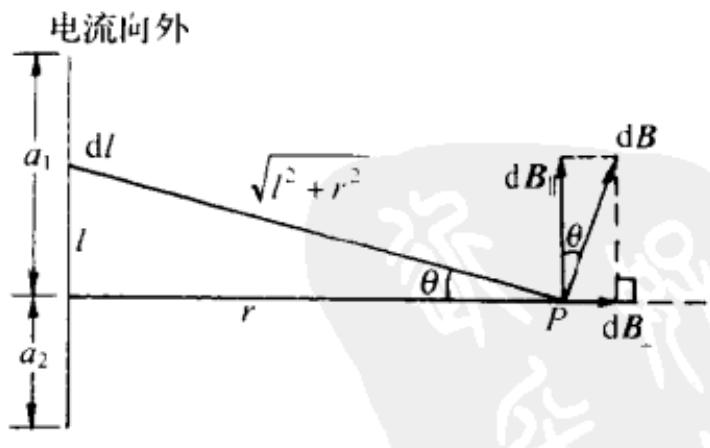
\includegraphics[width=0.5\linewidth]{figures/fig_5_1_40_2.jpg}
\end{center}

\vfill

\newpage

\textbf{5.1.41.} 一半径为 $R$ 的圆柱面上载有电流 $I, I$ 平行于圆柱面的轴线流动，并且均匀分布在圆柱面上。试求这圆柱面上任一点的磁感强度（即面电流所在处的磁感强度）。

\vfill

\textbf{5.1.42.} 电流 I 均匀分布在无穷长的半圆柱面上, 并平行于轴线流动, 圆柱面的半径为 R. 试求轴线上任一点的磁感强度 B, 并计算 $R = 1.0 \, cm, I = 5.0 \, A$ 时 B 的值.

\vfill

\newpage

\textbf{5.1.43.} 在一条长直导线旁放一个小磁针, 当导线里通有电流时, 小磁针便会偏转. 根据计算, 这时导线里的自由电子以平均定向速度 u 沿导线移动. 如果令这小磁针也以速度 u 平行于导线移动, 试问小磁针是否偏转? 为什么?

【解答】小磁针会偏转,而且是相同的偏转.这是因为,在跟随小磁针运动的参考系里,自由电子虽然相对静止,但导线里的正电荷却以-u运动,这种运动所产生的电流与在相对于导线静止的参考系中所观测到的电流相同.因此,在跟随小磁针运动的参考系里和在相对于导线静止的参考系里,导线中的电流所产生的磁场相同.所以小磁针的偏转也相同.

\vfill

\textbf{5.1.44.} 氢原子处在基态时,根据经典模型,它的电子在半径为 $a = 0.529 \times 10^{-8} ~cm$ 的轨道(玻尔轨道)上作匀速圆周运动,速率为 $v = 2.19 \times 10^{8} ~cm/s$ ,已知电子电荷的大小为 $e = 1.60 \times 10^{-19} ~C$ .试求电子的这种运动在轨道中心产生的磁感强度 B 的值.

\vfill

\newpage

\textbf{5.1.45.} 根据经典模型, 原子里的电子绕原子核作圆周运动。(1)试证明: 这种轨道运动所产生的磁矩 m 与它的角动量 L 的关系为 $m = -\frac{e}{2m_{e}}L$ , 式中 $m_{e}$ 是电子的质量, e 是电子电荷的大小; (2) L 的大小一般是 $h = 1.054573 \times 10^{-34} J \cdot s$ 的数量级, 通常把 $m_{B} = \frac{e\hbar}{2m_{e}}$ 叫做玻尔磁子, 是原子磁矩的一种单位. 已知 $m_{e} = 9.10939 \times 10^{-31} kg$ , $e = 1.602177 \times 10^{-19} C$ . 试计算玻尔磁子的值.

\vfill

\textbf{5.1.46.} 电荷量 q 均匀地分布在半径为 R 的圆环上, 这环以匀角速度 $\omega$ 绕它的几何轴旋转, 如图 5.1.46 所示. 试求: (1) 轴线上离环心 O 为 r 处的磁感强度 B; (2) 磁矩 m.

\vfill

\newpage

\textbf{5.1.47.} 半径为 R 的圆片上均匀带电, 电荷量的面密度为 $\sigma$ , 这圆片以匀角速角 $\omega$ 绕它的几何轴旋转, 如图 5.1.47 所示. 设片的厚度可略去不计, 试求: (1) 轴线上离圆心为 r 处的磁感强度 B; (2) 磁矩 m.

\vfill

\textbf{5.1.48.} 电荷量 $Q$ 均匀地分布在半径为 $R$ 的球面上, 这球面以匀角速度 $\omega$ 绕它的一个固定的直径旋转. 试求: (1) 轴线上离球心为 $r$ 处的磁感强度 $\pmb{B}$ ; (2) 磁矩 $\pmb{m}$ .

图 5.1.48(1)
\begin{center}
    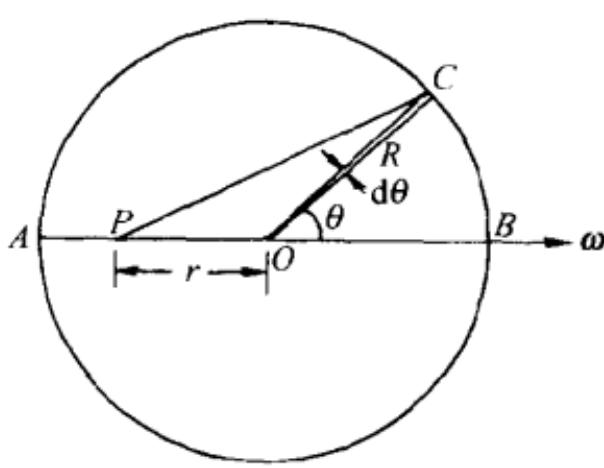
\includegraphics[width=0.5\linewidth]{figures/fig_5_1_48.jpg}
\end{center}

\vfill

\newpage

\textbf{5.1.49.} 电荷量 Q 均匀地分布在半径为 R 的球体内, 这球体以匀角速度 $\omega$ 绕它的一个固定的直径旋转. 试求: (1) 球内离转轴为 r 处电流密度 j 的大小; (2) 轴线上离球心为 r 处的磁感强度 B; (3) 磁矩.

\vfill

\textbf{5.1.50.} 一个球形的铀块 $^{(238}\mathrm{U)}$ 均匀地向四面八方放射出带正电的 $\alpha$ 粒子，每秒钟共放射出N个 $\alpha$ 粒子，每个 $\alpha$ 粒子的电荷量均为2e.试求离球心为r处的电流密度 $j(r)$ 和磁感强度 $B(r)$ .

\vfill

\newpage

\textbf{5.2.1.} 一般教科书上推导安培环路定理,都是以无限长直载流导线为例,在

图5.2.1

垂直于导线的平面内作环路. 如果环路不限定在上述平面内, 你能否推导出同样结果?
\begin{center}
    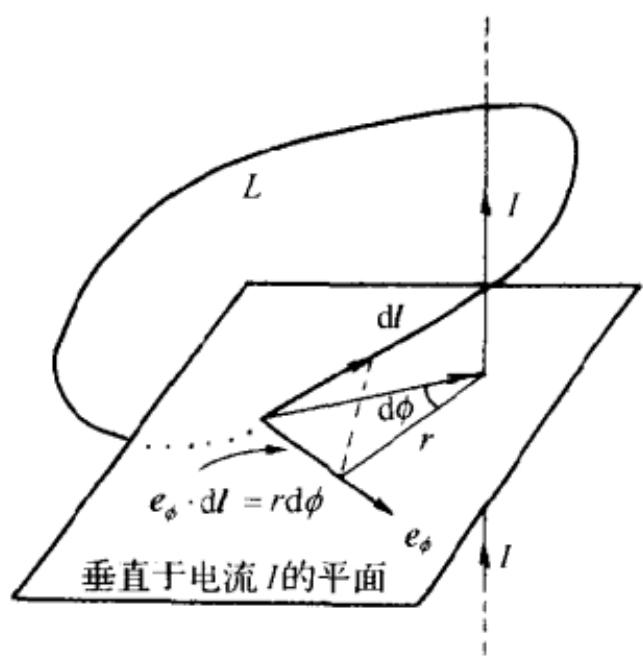
\includegraphics[width=0.5\linewidth]{figures/fig_5_2_1.jpg}
\end{center}

\vfill

\textbf{5.2.2.} 两条无穷长的平行直导线相距为 $2a$ ，分别载有方向相同的电流 $I_{1}$ 和 $I_{2}$ ；空间任一点 $P$ 到 $I_{1}$ 的垂直距离为 $r_{1}$ ，到 $I_{2}$ 的垂直距离为 $I_{2}$ ，如图5.2.2(1)所

示. 试求 P 点的磁感强度 B.

\vfill

\newpage

\textbf{5.2.3.} 两条无穷长的平行直导线相距为 a，载有大小相等而方向相反的电流 I；空间任一点 P 到两导线的垂直距离分别为 $r_{1}$ 和 $r_{2}$ ，如图 5.2.3(1) 所示。试求 P 点的磁感强度 B。

\vfill

\textbf{5.2.4.} 两条无穷长的平行直导线相距为 $a$ ，载有大小相等而方向相反的电流 $I$ ；在这两导线构成的平面内有一点 $P, P$ 到其中一导线的距离为 $r$ 。试求 $P$ 点的磁感强度 $\pmb{B}$ 。

图5.2.4
\begin{center}
    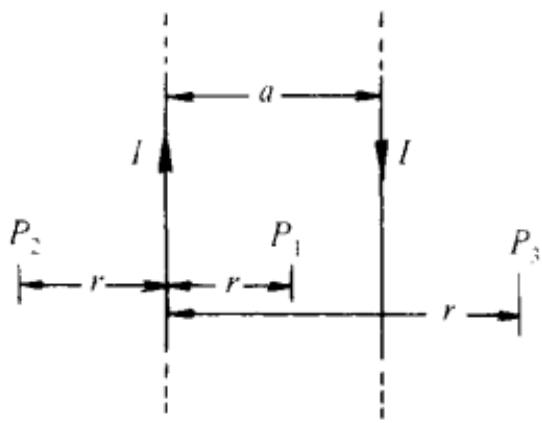
\includegraphics[width=0.5\linewidth]{figures/fig_5_2_4.jpg}
\end{center}

\vfill

\newpage

\textbf{5.2.5.} 四条无穷长的平行直导线,它们的横截面是边长为 a 的正方形,每条导线中的电流都是 I,它们的方向如图 5.2.5 所示.试求正方形中心的磁感强度 B;并计算 $a=20cm, I=20A$ 时 B 的值.

\vfill

\textbf{5.2.6.} 两条无穷长直导线互相垂直而不相交,其间最近距离为 a=2.0cm,电流分别为 $I_{1}=4.0A$ 和 $I_{2}=6.0A$ . P 点到两导线的垂直距离都是 a,如图 5.2.6 所示.试求 P 点的磁感强度 B.
\begin{center}
    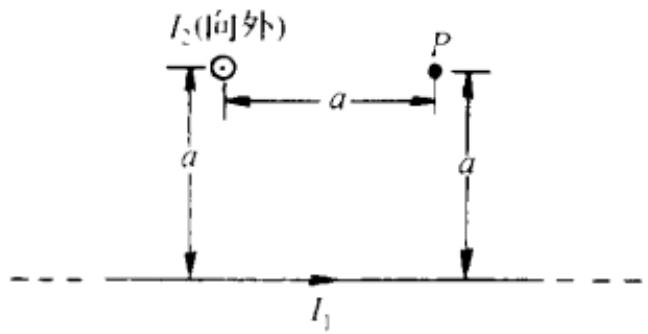
\includegraphics[width=0.5\linewidth]{figures/fig_5_2_6.jpg}
\end{center}

\vfill

\newpage

\textbf{5.2.7.} 一无穷长直线电流 I 沿 z 轴向下流到坐标原点, 然后在 x - y 平面上
均匀地散开, 向各个方向直流向无穷远去, 如图 5.2.7 所示. 试求空间各处的磁感强度.

\vfill

\textbf{5.2.8.} 一载有电流 I 的无穷长直导线垂直到地面, I 到达地面后, 便分散开来, 均匀地向各个方向流去, 如图 5.2.8(1) 所示. 把地面当作无穷大的平面, 设大地的磁导率为 $\mu_{0}$ , 试求地面以上和地面以下各处的磁感强度.

\vfill

\newpage

\textbf{5.2.9.} 一无穷大平面上有均匀分布的电流, 面电流密度为 k, k 的方向是电流流动的方向, k 的大小等于通过单位长度(该面上垂直于 k 的单位长度)的电流. 试求这面电流在离它为 r 处产生的磁感强度 B.

图 5.2.9(1)
\begin{center}
    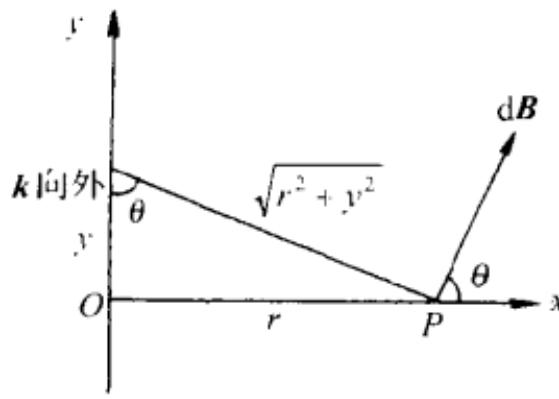
\includegraphics[width=0.5\linewidth]{figures/fig_5_2_9.jpg}
\end{center}

\vfill

\textbf{5.2.10.} 两无穷大的平行平面上都有均匀分布的电流，面电流密度分别为 $k_{1}$ 和 $k_{2}, k_{1}$ 与 $k_{2}$ 平行，它们的一部分如图5.2.10所示。(1)试求两面之间的磁感强度 $\pmb{B}$ ; (2)试求两面之外的磁感强度 $\pmb{B}$ ; (3)当 $k_{1} = k_{2}$ 时结果如何？(4)当 $k_{1} = -k_{2}$ 时结果如何？

图5.2.10

\vfill

\newpage

\textbf{5.2.11.} 两无穷大的平行平面上都有均匀分布的电流, 面电流密度分别为 $k_{1}$ 和 $k_{2}, k_{1}$ 和 $k_{2}$ 的夹角为 $\theta$ . (1) 试求两面之间的磁感强度; (2) 试求两面之外的磁感强度; (3) 当 $\theta = \pi$ , 且 $|k_{1}| = |k_{2}|$ 时, 结果如何?

\vfill

\textbf{5.2.12.} 电流 I 均匀分布在半径为 R 的无限长直圆筒面上, 平行于圆筒的轴线流动. 试求这电流在离轴线为 r 处产生的磁感强度 B.

\vfill

\newpage

\textbf{5.2.13.} 一无穷长的导体直圆管,内半径为 a,外半径为 b,载有电流 I,I 沿轴线方向流动,并且均匀分布在圆管的横截面上,其中一段如图 5.2.13 所示.试求离管的轴线为 r 处的磁感强度 B.
\begin{center}
    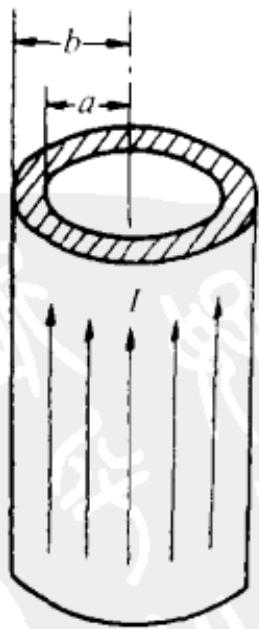
\includegraphics[width=0.5\linewidth]{figures/fig_5_2_13.jpg}
\end{center}

\vfill

\textbf{5.2.14.} 一很长的导体直圆管, 管厚为 $5.0 \mathrm{~mm}$ , 外直径为 $50.0 \mathrm{~mm}$ , 载有 50A 的电流, 电流沿管的轴线方向流动, 并且均匀分布在管的横截面上. 试求下列几处磁场强度 $\pmb{H}$ 的大小 $H$ : (1) 管外靠近外壁; (2) 管内靠近内壁; (3) 内外壁之间的中点.

\vfill

\newpage

\textbf{5.2.15.} 一很长的直同轴电缆,里面导线的半径为 a,外面是半径为 b 的导体薄圆管,其厚度可略去不计.电流 I 由导线流去,由圆管流回,并均匀分布在导线和管的横截面上. 试求离轴线为 r 处的磁感强度 B 的大小.

\vfill

\textbf{5.2.16.} 电缆由一导体圆柱和一同轴导体圆管构成,使用时,电流 I 从一导体流去,由另一导体流回,电流都是均匀分布在横截面上.已知圆柱的半径为 $r_{1}$ , 圆管的内外半径分别为 $r_{2}$ 和 $r_{3}$ , 其中一段如图 5.2.16 所示.试求离轴线为 r 处的磁场强度 H 的大小.

\vfill

\newpage

\textbf{5.2.17.} 半径为 R 的无穷长直圆柱面上有一层均匀分布的面电流, 电流都环绕着轴线流动并与轴线垂直(图 5.2.17(1)), 面电流密度为 k, k 的大小等于通过单位长度(该面上垂直于 k 的单位长度)的电流. 试求离轴线为 r 处的磁感强度 B.

\vfill

\textbf{5.2.18.} 半径为 R 的无穷长直圆柱面上有一层均匀分布的面电流, 电流都环绕轴线流动并与轴线方向成一角度 $\theta$ , 即电流在圆柱面上沿螺旋线向前流动, 其中一段如图 5.2.18 所示. 已知面电流密度为 k, k 的方向为螺旋线的切线方向, k 的大小等于通过单位长度(该面上垂直于 k 的单位长度)的电流. 试求离轴线为 r 处的磁感强度.
\begin{center}
    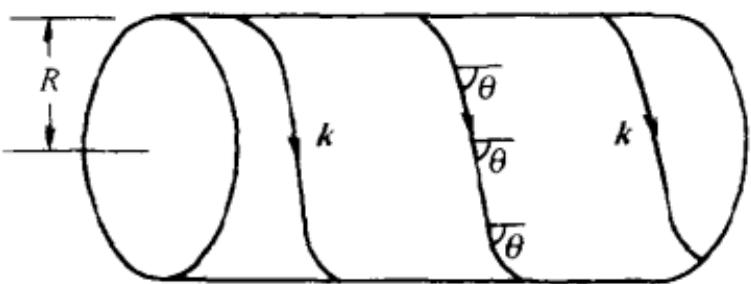
\includegraphics[width=0.5\linewidth]{figures/fig_5_2_18.jpg}
\end{center}

\vfill

\newpage

\textbf{5.2.19.} 一螺绕环由表面绝缘的细导线密绕而成, 共有 N 匝, 中间的半径为 R, 横截面是半径为 r 的圆形, 如图 5.2.19 所示, 已知 $r \ll R$ . 当导线中载有电流 I 时, 试求环内磁感强度的大小 B.

\vfill

\textbf{5.2.20.} 试证明：无限长密绕螺线管载

有电流时,管内磁场是均匀磁场.

\vfill

\newpage

\textbf{5.2.21.} 电荷量 $Q$ 均匀分布在半径为 $R$ 的球面上，这球面以匀角速度绕它的一个固定直径旋转。试论证球内磁场是均匀磁场。

【论证】将球面上的旋转电荷当作是许多圆电流，根据圆电流在轴线上产生磁感强度的公式，可以算出球面内轴线上每一点的磁感强度均为[参见前面5.1.48题的式(7)]

$$
\boldsymbol {B} = \frac {\mu_ {0} Q}{6 \pi R} \boldsymbol {\omega}\tag{1}
$$

式中 R 是球面的半径, $\omega$ 是角速度.

如图5.2.21(1)，设 $c, d, O, e, f$ 为轴线 $ab$ 上的几点，其中 $O$ 为球心，则有

$$
B _ {c} = B _ {d} = B _ {O} = B _ {e} = B _ {f} = \frac {\mu_ {0} Q \omega}{6 \pi R}\tag{2}
$$

根据轴对称性,球面内的 B 线只有三种可能性,分别如图 5.2.21(2)、(3) 和 (4) 所示. 先看图 (2),其中 B 线在球心处最密集,故轴线 ab 上各点的磁感强度的值应有

(1)


(3)

(2)
(4)
图5.2.21

$$
B _ {c} <   B _ {d} <   B _ {O}, \quad B _ {O} > B _ {e} > B _ {f}\tag{3}
$$

式(3)不满足式(1)，所以球面内的 B 线不能是图 5.2.21(2)的形状。再看图 5.2.21(3)，其中 B 线在球心处最松散，故轴线 ab 上各点的磁感强度的值应有

$$
B _ {c} > B _ {d} > B _ {O}, \quad B _ {O} <   B _ {e} <   B _ {f}\tag{4}
$$

式(4)也不满足式(1)，所以球面内的 B 线也不能是图 5.2.21(3) 的形状.

于是我们得出结论:球面内的 B 线只能是图 5.2.21(4) 的形状,即平行于轴线的直线.

图 5.2.21(5)

再由安培环路定理证明球内磁场是均匀磁场. 如图 5.2.21(5), 设在球内任一点 P, 磁感强度为 B; 取长方形安培环路 L, 边长为 l 的一边在轴线上, 其对边通过 P 点, 则有

所以

$$
\oint_ {L} \boldsymbol {B} \cdot \mathrm{d} \boldsymbol {l} = B _ {0} l - B l = 0
$$

$$
B = B _ {0}\tag{5}
$$

(6)

这表明球内任一点的磁感强度都等于球心的磁感强度.
\begin{center}
    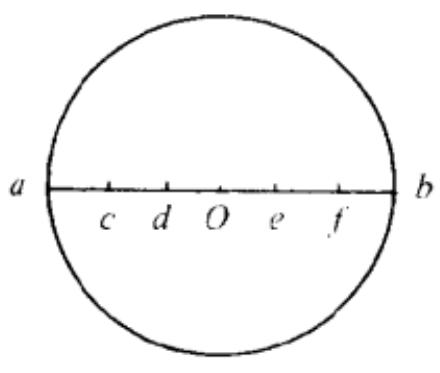
\includegraphics[width=0.5\linewidth]{figures/fig_5_2_21_1.jpg}
\end{center}
\begin{center}
    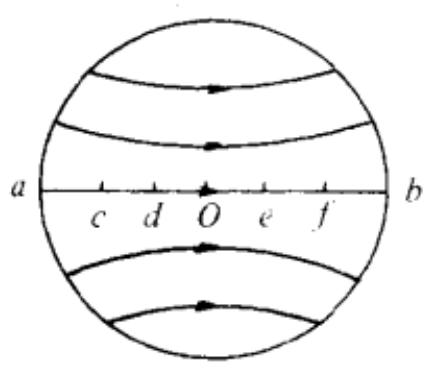
\includegraphics[width=0.5\linewidth]{figures/fig_5_2_21_2.jpg}
\end{center}
\begin{center}
    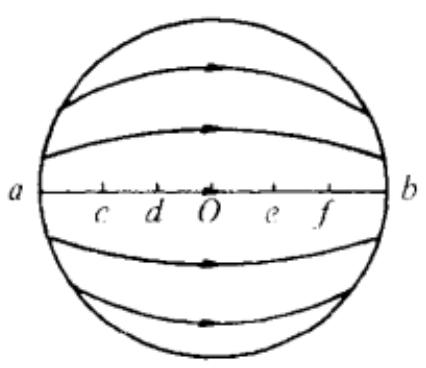
\includegraphics[width=0.5\linewidth]{figures/fig_5_2_21_3.jpg}
\end{center}
\begin{center}
    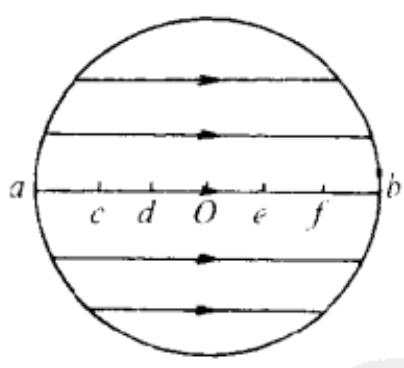
\includegraphics[width=0.5\linewidth]{figures/fig_5_2_21_4.jpg}
\end{center}
\begin{center}
    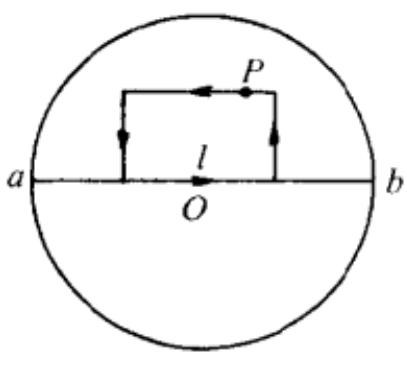
\includegraphics[width=0.5\linewidth]{figures/fig_5_2_21_5.jpg}
\end{center}

\vfill

\textbf{5.2.22.} 一载有电流 I 的无穷长直导线, 半径为 a, I 均匀分布在横截面上, 图 5.2.22 是这导线纵剖面的一部分,

其中 ABCD 是一个长方形, AB 边在轴线上, CD 边在表面上, CD = l. 试求通过 ABCD 的磁通量.

\vfill

\newpage

\textbf{5.2.23.} 半径为 R 的无穷长直圆柱形导体, 载有沿轴线方向流动的电流, 电流均匀分布在横截面上, 电流密度为 j. 试求离导体轴线为 r 处的磁感强度.

\vfill

\textbf{5.2.24.} 外半径为 R 的无穷长圆柱形导体管, 管内空心部分的半径为 r, 空心部分的轴线与圆柱的轴线平行, 但不重合, 相距为 a, 管的一段如图 5.2.24 所示. 今有电流 I 沿轴线方向流动, I 均匀分布在管的横截面上. (1) 试分别求圆柱轴线上和空心轴线上的磁感强度 B 的大小 B. (2) 当 R = 1.0cm, r = 0.5mm, a = 5.0mm 和 I = 31A 时, 试计算上述两处 B 的值.

\vfill

\newpage

\textbf{5.2.25.} 一无限长直圆柱体,内有一无限长直圆柱形空洞,空洞的轴线与圆柱的轴线平行但不重合,相距为 a. 今有电流沿轴线方向流动并均匀分布在横截面上,电流密度为 j. 试证明:洞内的磁场是均匀磁场,并求出它的磁感强度.

图5.2.25
\begin{center}
    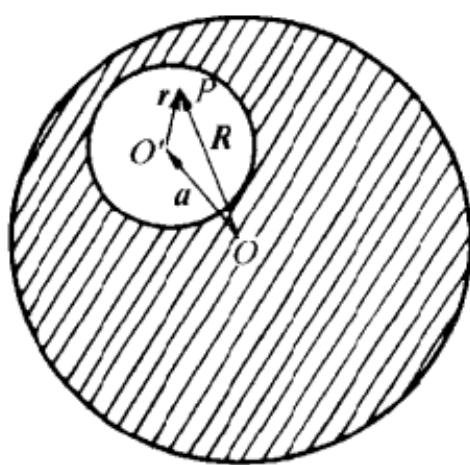
\includegraphics[width=0.5\linewidth]{figures/fig_5_2_25.jpg}
\end{center}

\vfill

\textbf{5.2.26.} 电流沿圆柱形长导线流动,导线内离轴线为 r 处,电流密度的大小 j 和磁场强度的大小 H 都是 r 的函数.试证明: $j=\frac{H}{r}+\frac{\partial H}{\partial r}$ .

\vfill

\newpage
